\scanpage{40}
\mspage{32}
% L1–5
Considérons les 6 \deleted{\unsure{racines|racines, et}} \inserted{bases} orth. à un bitriangle $(u,v,w,\ u'=\alpha_4,v'=\beta_4,w'=\gamma_4,u''=\alpha'_{\unsure{4|2|1}},v''=\beta'_4,w''=\gamma'_4)$ \deleted{\unsure{dans le}} avec les notations des pp. 9, 10. On trouve les bases \deleted{de la forme}
% L6–11
\[
b=(\alpha_1,\alpha'_2,\beta_1,\beta'_2,\gamma_1,\gamma'_2)
\]
et celles qui s'en déduisent par les \inserted{6} permutations de $\{1,2,3\}$. La base duale à la base écrite est $b'=(\alpha_2,\alpha'_1,\beta_{\unsure{2|3}},\beta'_1,\gamma_2,\gamma'_1)$, la racine correspondante à $b$ est
\[
\alpha_2-\alpha_1=\alpha'_1-\alpha'_2=\beta_2-\beta_1=\beta'_1-\beta'_2=\gamma_2-\gamma_1=\gamma'_1-\gamma'_2,
\]
% L12–15
on trouve donc les 6 racines de la forme $\alpha_i-\alpha_j$ $(i\ne j,\ 1\le i,j\le3)$. Elles forment évidemment un \uline{syst. de racines de type $A_2$}

\figure{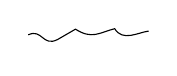
\begin{tikzpicture}[scale=.6]\draw (0,0)..controls (.3,.14) and (.3,-.26)..(.62,-.10)--(1,.12)..controls (1.35,-.1) and (1.49,.04)..(1.83,.13)..controls (2,-.15) and (2.32,.05)..(2.55,.08);\end{tikzpicture}}
% L16–19
expliciter a) les positions relatives d'un bitriangle \inserted{$\Delta$} et d'un triangle $t$. Il y en a trois
\[
\left\{\begin{aligned}
&t\subset\Delta\quad\text{i.e. }\operatorname{card}t\cap\Delta=3\\
&\operatorname{card}(t\cap\Delta)=1\\
&\deleted{\unsure{t\in}}t\cap\Delta=\varnothing\quad\text{i.e. }\operatorname{card}(t\cap\Delta)=0
\end{aligned}\right.
\quad\begin{array}{|r}6\\3\cdot9\\12\\\hline\hline45\end{array}
\]
% L20–25
b) Les positions relatives d'une base (ou bibase) et d'un bitriangle (il semble qu'il y en ait trois : $b$ orthogonale à $\Delta$, $b$ \inserted{non orth. à $\Delta$ mais} orthogonale à au moins un triangle de $\Delta$ (Alors il est \unsure{orth.} à \unsure{exactt|exactement} 2 triangles \unsure{dont|et dont} la réunion est de cardinal 5 \ldots), enfin $b$ orth. à aucun triangle de $\Delta$\ldots
% margin note written sideways
\margin{c) positions relatives de deux bitriangles ???}
% archive sheet number: 39
